\documentclass[10pt,a4paper]{article}
\usepackage[utf8]{inputenc}
\usepackage[T1]{fontenc}
\usepackage{amsmath}
\usepackage{amsfonts}
\usepackage{amssymb}
\usepackage{makeidx}
\usepackage{graphicx}

% More defined colors
\usepackage[dvipsnames]{xcolor}

% Required package
\usepackage{tikz}
\usetikzlibrary{positioning}

\usepackage[left=1.00in, right=1.00in, top=1.00in, bottom=1.00in]{geometry}
\author{Tommaso Severini}
\title{Chimica - Composti binari}

\parindent 0ex
\begin{document}
	\maketitle
	
	I composti binari, ovvero la classe di composti inorganici contenenti unicamente 2 specie chimiche, si possono classificare a seconda del legame che unisce le specie chimiche:\\
	
\textbf{	Legame ionico:}
	
	\begin{itemize}
		\item Idruri metallici (gruppi 1 e 2)
		\item Ossidi basici (metallici)
		\item Sali binari
	\end{itemize}

\textbf{	Legame covalente:}
	
	\begin{itemize}
		\item Idruri covalenti (non metalli/semimetalli gruppi 14, 15, 16)
		\item Ossidi acidi (non metalli/semimetalli)
		\item Idracidi (non metalli)
	\end{itemize}

\section*{Composti dell'idrogeno}

 \subsection*{Idracidi}
 
 	Gli idracidi (o acidi alogenidrici) sono composti binari dell'idrogeno con i non metalli (gruppi 16 e 17). L'idrogeno in questi composti ha \textbf{numero di ossidazione +1}.\\
 	
 	\begin{tabular}{|c|c|c|}
 		\hline
 		Formula chimica & Nomenclatura tradizionale & Nomenclatura IUPAC \\
 		\hline
 		Idrogeno + non metallo & acido + nonmetallo -idrico & nonmetallo -uro + di + n-idrogeno \\
 		\hline
 	\end{tabular} \\
 
 	Ad esempio, il composto HCl prende, tradizionalmente il nome "acido cloridrico", il nome di "cloruro di (mono)idrogeno".
 	
 	Una delle più notabili eccezioni è costituita dai composti del cianuro (CN). Infatti, nonostante esso si composto da 2 specie chimiche elementari, è spesso considerato come una specie unica. Per questo motivo il composto HCN prende, tradizionalmente il nome "acido cianidrico", il nome "cianuro di idrogeno".
 	
 \subsection*{Idruri}
 
	Gli idruri sono composti in cui l'idrogeno si lega con uno dei metalli (o semimetalli o non metalli) dei gruppi 1 a 15. In questi composti, l'idrogeno tende ad avere \textbf{numero di ossidazione -1}.\\
	
	\begin{tabular}{|c|c|c|}
		\hline
		Formula chimica & Nomenclatura tradizionale & Nomenclatura IUPAC \\
		\hline
		Metallo*  + idrogeno & Idruro di + metallo*  & N-idruro + di metallo*  \\
		\hline
	\end{tabular}\\
	
	*per i semimetalli ed i non metalli la nomenclatura rimane invariata.
	
\section*{Composti dell'ossigeno}

	Vengono definiti ossidi tutti quei composti binari che contengono l'ossigeno.
	
	Formula chimica: $X_mO_n$, dove $X$ è un elemento qualsiasi della tavola periodica.
	
	Gli ossidi possono essere suddivisi in tre classi in base al numero di ossidazione che presenta l'ossigeno:\\
	
	Ossidi: n.o. = -2 \hfill
	Perossidi: n.o. = -1\hfill
	Superossidi: n.o. = -0.5
		
	
\section*{Nomenclatura tradizionale degli ossidi}

\begin{center}
	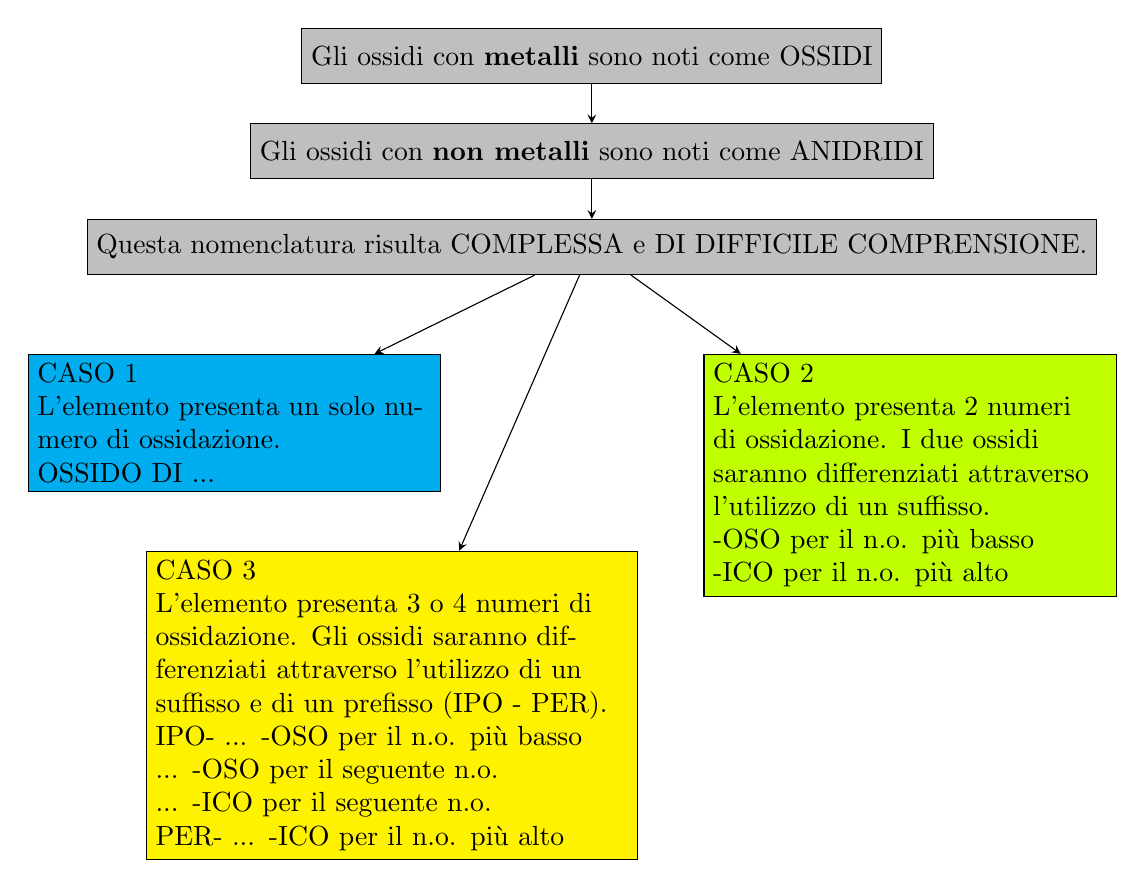
\begin{tikzpicture}
		
		
		% Controller
		\node [draw,
		fill=lightgray,
		minimum width=2cm,
		minimum height=0.7cm,
		]  (intro0) {Gli ossidi con \textbf{metalli} sono noti come OSSIDI};
	
		% Sensor block
		\node [draw,
		fill=lightgray, 
		minimum width=2cm, 
		minimum height=0.7cm, 
		below= 0.5cm of intro0
		]  (intro1) {Gli ossidi con \textbf{non metalli} sono noti come ANIDRIDI};
		
		\node [draw,
		fill=lightgray, 
		minimum width=2cm, 
		minimum height=0.7cm, 
		below= 0.5cm of intro1
		]  (intro2) {Questa nomenclatura risulta COMPLESSA e DI DIFFICILE COMPRENSIONE.};
		
		\node [draw,
		fill=cyan, 
		minimum width=2cm,
		text width=5cm, 
		minimum height=0.7cm, 
		below left= 1cm and -4.5cm of intro2
		]  (caso1) {CASO 1\\
			
			L'elemento presenta un solo numero di ossidazione. \\
		
		OSSIDO DI ...};
	
		\node [draw,
		fill=lime, 
		minimum width=2cm,
		text width=5cm, 
		minimum height=0.7cm, 
		below right= 1cm and -5cm of intro2
		]  (caso2) {CASO 2\\
			
			L'elemento presenta 2 numeri di ossidazione. I due ossidi saranno differenziati attraverso l'utilizzo di un suffisso.\\
			
			-OSO per il n.o. più basso\\
		
			-ICO per il n.o. più alto};	
		
		\node [draw,
		fill=yellow, 
		minimum width=2cm,
		text width=6cm, 
		minimum height=0.7cm, 
		below left= 3.5cm and -7cm of intro2
		]  (caso3) {CASO 3\\
			
			L'elemento presenta 3 o 4 numeri di ossidazione. Gli ossidi saranno differenziati attraverso l'utilizzo di un suffisso e di un prefisso (IPO - PER).\\
			
			IPO- ... -OSO per il n.o. più basso\\
			
			... -OSO per il seguente n.o.\\
			
			... -ICO per il seguente n.o.\\
			
			PER- ... -ICO per il n.o. più alto};
		
		\draw[-stealth] (intro0) -- (intro1);
		
		\draw[-stealth] (intro1) -- (intro2);
		
		\draw[-stealth] (intro2) -- (caso1);
		
		\draw[-stealth] (intro2) -- (caso2);
		
		\draw[-stealth] (intro2) -- (caso3);
		
		\end{tikzpicture}
	
\end{center}

	\section*{Sali binari}
	
	Vengono definiti sali tutti quei composti che presentano un legame ionico e che quindi comprendono una parte metallica, scritta per prima nella formula chimica, e una non metallica, scritta per seconda nella formula chimica.\\
	
	\begin{tabular}{|c|c|c|}
		\hline
		Formula chimica & Nomenclatura tradizionale & Nomenclatura IUPAC \\
		\hline
		metallo + non metallo & non metallo-uro + di + metallo* & n-non metallo-uro + di + n-metallo \\
		\hline
	\end{tabular}\\

	*nel caso il metallo presenti più numeri di ossidazione, sarà necessario utilizzare i suffissi -OSO (n.o. più basso) e -ICO (n.o. più alto).
	
	
\end{document}